
\definecolor{cc6d4dc}{RGB}{198,212,220}
\definecolor{cffffff}{RGB}{255,255,255}
\definecolor{cfffde8}{RGB}{255,253,232}


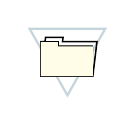
\begin{tikzpicture}[y=0.80pt, x=0.80pt, yscale=-1.000000, xscale=1.000000, inner sep=0pt, outer sep=0pt]
\begin{scope}% layer1
  \begin{scope}[shift={(140.43014,284.01592)}]% g3477
    \begin{scope}% g3479
      % path3481
      \path[fill=cc6d4dc] (22.4280,38.3980) -- (4.4730,6.8660) -- (40.3810,6.8660) --
        (22.4280,38.3980) -- (22.4280,38.3980) -- cycle(6.1940,7.8660) --
        (22.4280,36.3780) -- (38.6610,7.8660) -- (6.1940,7.8660) -- (6.1940,7.8660) --
        cycle;

    \end{scope}
    \begin{scope}% g3483
      \begin{scope}% g3485
        % polygon3487
        \path (12.5550,11.2050) -- (20.4470,11.2050) -- (20.2110,13.1740) --
          (35.7710,13.1580) -- (33.8980,28.7910) -- (10.4490,28.7910) --
          (10.4490,13.1580) -- (12.3220,13.1580) -- cycle;

        % polygon3489
        \path[draw=black,miter limit=3.86,line width=0.552pt] (12.5550,11.2050) --
          (20.4470,11.2050) -- (20.2110,13.1740) -- (35.7710,13.1580) --
          (33.8980,28.7910) -- (10.4490,28.7910) -- (10.4490,13.1580) --
          (12.3220,13.1580) -- cycle;

      \end{scope}
      \begin{scope}% g3491
        % polygon3493
        \path[fill=cffffff] (18.3410,15.1280) -- (33.8980,15.1130) -- (33.8980,28.7910)
          -- (10.4490,28.7910) -- (10.4490,13.1580) -- (18.3410,13.1580) -- cycle;

        % polygon3495
        \path[draw=black,miter limit=3.86,line width=0.276pt] (18.3410,15.1280) --
          (33.8980,15.1130) -- (33.8980,28.7910) -- (10.4490,28.7910) --
          (10.4490,13.1580) -- (18.3410,13.1580) -- cycle;

      \end{scope}
      \begin{scope}% g3497
        % polyline3499
        \path[draw=black,miter limit=3.86,line width=0.276pt] (10.4540,13.1580) --
          (18.3410,13.1580) -- (18.3410,15.1280) -- (33.8980,15.1130);

      \end{scope}
      \begin{scope}% g3501
        % line3503
        \path[draw=black,miter limit=3.86,line width=0.135pt] (12.4020,19.0200) --
          (26.0830,19.0200);

      \end{scope}
      \begin{scope}% g3505
        % line3507
        \path[draw=black,miter limit=3.86,line width=0.135pt] (12.4020,20.9740) --
          (26.0830,20.9740);

      \end{scope}
      \begin{scope}% g3509
        % line3511
        \path[draw=black,miter limit=3.86,line width=0.135pt] (12.4020,22.9280) --
          (26.0830,22.9280);

      \end{scope}
      \begin{scope}% g3513
        % polygon3515
        \path[fill=cfffde8] (18.3410,15.1280) -- (33.8980,15.1130) -- (33.8980,28.7910)
          -- (10.4490,28.7910) -- (10.4490,13.1580) -- (18.3410,13.1580) -- cycle;

        \begin{scope}% g3517
          % path3519
          \path (34.0710,28.9620) -- (10.2770,28.9620) -- (10.2770,12.9850) --
            (18.5130,12.9850) -- (18.5130,14.9560) -- (34.0710,14.9400) --
            (34.0710,28.9620) -- (34.0710,28.9620) -- cycle(10.6220,28.6190) --
            (33.7260,28.6190) -- (33.7260,15.2850) -- (18.1680,15.3010) --
            (18.1680,13.3300) -- (10.6210,13.3300) -- (10.6220,28.6190) --
            (10.6220,28.6190) -- cycle;

        \end{scope}
      \end{scope}
      \begin{scope}% g3521
        % polyline3523
        \path[draw=black,miter limit=3.86,line width=0.276pt] (10.4540,13.1580) --
          (18.3410,13.1580) -- (18.3410,15.1280) -- (33.8980,15.1130);

      \end{scope}
      \begin{scope}% g3525
        \begin{scope}% g3527
          % polygon3529
          \path (12.4020,18.9360) -- (26.0830,18.9360) -- (26.0830,19.1040) --
            (12.4020,19.1040) -- cycle;

        \end{scope}
      \end{scope}
      \begin{scope}% g3531
        \begin{scope}% g3533
          % polygon3535
          \path (12.4020,20.8900) -- (26.0830,20.8900) -- (26.0830,21.0590) --
            (12.4020,21.0590) -- cycle;

        \end{scope}
      \end{scope}
      \begin{scope}% g3537
        \begin{scope}% g3539
          % polygon3541
          \path (12.4020,22.8440) -- (26.0830,22.8440) -- (26.0830,23.0130) --
            (12.4020,23.0130) -- cycle;

        \end{scope}
      \end{scope}
    \end{scope}
  \end{scope}
\end{scope}

\end{tikzpicture}
